\documentclass[conference]{IEEEtran}

% graphic declaration
\usepackage{graphicx}
\usepackage{listings}
\usepackage[english]{babel}
\usepackage{float}
\usepackage{color}

\definecolor{dkgreen}{rgb}{0,0.6,0}
\definecolor{gray}{rgb}{0.5,0.5,0.5}
\definecolor{mauve}{rgb}{0.58,0,0.82}

\lstset{frame=tb,
  language=Java,
  aboveskip=3mm,
  belowskip=3mm,
  showstringspaces=false,
  columns=flexible,
  basicstyle={\footnotesize\ttfamily},
  numbers=none,
  numberstyle=\tiny\color{gray},
  keywordstyle=\color{blue},
  commentstyle=\color{dkgreen},
  stringstyle=\color{mauve},
  breaklines=true,
  breakatwhitespace=true,
  tabsize=3
}

\graphicspath{ {data/} }

\ifCLASSINFOpdf
  % \usepackage[pdftex]{graphicx}
  % declare the path(s) where your graphic files are
  % \graphicspath{{../pdf/}{../jpeg/}}
  % and their extensions so you won't have to specify these with
  % every instance of \includegraphics
  % \DeclareGraphicsExtensions{.pdf,.jpeg,.png}
\else
  % or other class option (dvipsone, dvipdf, if not using dvips). graphicx
  % will default to the driver specified in the system graphics.cfg if no
  % driver is specified.
  % \usepackage[dvips]{graphicx}
  % declare the path(s) where your graphic files are
  % \graphicspath{{../eps/}}
  % and their extensions so you won't have to specify these with
  % every instance of \includegraphics
  % \DeclareGraphicsExtensions{.eps}
\fi

% correct bad hyphenation here
\hyphenation{op-tical net-works semi-conduc-tor}


\begin{document}
%
% paper title
% Titles are generally capitalized except for words such as a, an, and, as,
% at, but, by, for, in, nor, of, on, or, the, to and up, which are usually
% not capitalized unless they are the first or last word of the title.
% Linebreaks \\ can be used within to get better formatting as desired.
% Do not put math or special symbols in the title.
\title{Job2P: Job Scheduling APIs for\\Wi-Fi Peer-to-peer Mobile Network}


% author names and affiliations
% use a multiple column layout for up to three different
% affiliations
\author{\IEEEauthorblockN{Le Dinh Minh}
\IEEEauthorblockA{Utah State University\\
ledinhminh3883@gmail.com}
\and
\IEEEauthorblockN{Young-Woo Kwon}
\IEEEauthorblockA{Utah State University\\
young.kwon@usu.edu}}


% make the title area
\maketitle

\begin{abstract}
These days, along with the rapid revolution of mobile device industry, software is also being built heavier and consumes more CPU performance and energy than they were in the past few years. Since the modern mobile devices support multiple connection methods like Wi-Fi, Bluetooth or NFC, the requirements of sharing the workloads and resources among the devices within a network to reduce full workload on an arbitrary device are being considered, especially in the areas Internet is not available, which can be found anywhere.

To address those limitations on mobile devices, we proposed Job2P as the Job Scheduling APIs for Android development that leverages Wi-Fi Direct to support sharing workloads and resources over peer-to-peer mobile device network, which doesn't require any Internet connections. Job2P provides a simple and straightforward API interface to get rid of sophistication of network implementation, letting developers easily create their distributed mobile applications with capability of forming closed range network. In term of workload distribution, Job2P splits task and resource into parts and packs them into the smaller units called jobs and dispatch to the peers. To distributed jobs equitably among the peers, a decision maker is added to decide the amount of resource the peer has to handle bases on its percentage of availability. Moreover, our APIs can handle fault tolerant for network malfunctions. 

Through our case studies, we realized that Job2P improves up to 45\% performance of running task in term of performance and energy consumption. 
\end{abstract}


% For peer review papers, you can put extra information on the cover
% page as needed:
% \ifCLASSOPTIONpeerreview
% \begin{center} \bfseries EDICS Category: 3-BBND \end{center}
% \fi
%
% For peerreview papers, this IEEEtran command inserts a page break and
% creates the second title. It will be ignored for other modes.
\IEEEpeerreviewmaketitle



\section{Introduction}
These days, mobile phones have been playing a very important role in human society. People need their cellphone everyday for surfing Internet, searching for information, online shopping, communicating with friends, taking and sharing photos etc. As a result of highly intensive completions between the global mobile phone manufactures like Samsung and Apple, the cellphones are more and more equipped themselves with high specifications (CPU, RAM and built-in storage) and top functionality so that they are powerful enough in compare with those in the past or even with a desktop. 

With the hardware rapid development, software is also being built more and more sophisticated in many aspects. They may occupy more space on local storage, use more memory, and thus consume more energy. Even though the software is designed to run on mobile device, its size may vary up to 1GB (like image processing or image recognizing) and memory consumption can be up to 1GB as well. Since there are possibly many heavy workloads running on a device at some points, the needs of sharing workloads among the mobile devices is really necessary with respect to performance and energy efficiency. 

Distributed computing are so far well-developed in PC or embedded networks, bringing the synthesized power of computation from multiple computers to solve a problem. Up to now, there are thousands of solutions for the developers to create a distributed computing system. For instance, the emergency of a number of message-oriented middleware like DataTurbine \cite{rbnb}, RabbitMQ \cite{rabbitmq} or NaradaBrokering \cite{naradabrokering} lessened the effort of development for distributed applications to the minimum but still maintained all equipped functionality like data mirroring, dynamic network topology or fault tolerant. However, despite of stunning equipments, it is revealed that the most disadvantage of this kind of applications is the dependence of network connection or wireless access point. Without a network established, nothing happens.

Unlike the other PCs or wired devices, the mobile devices have their own advantage of multiple non-equivalent network capability. One of the remarkable network capability is installed on modern mobile devices are Wi-Fi Direct, which allows them to discover the others in any short distance less than 200 meters without utilizing Internet and wireless access point. No internet connections are required, and it will help the owner to connect to the devices within a closed distance. By establishing connection between the two devices to form a pair, Wi-Fi Direct can provide the simple way to dynamically initiate a peer-to-peer network. Available on Android devices from version 4.0 (which more than 96\% of devices are using these days), as well as a number of Intel-featured laptops and game consoles, there is the high possibility of discovering the other mobile devices at anywhere.

To address those limitations with heavy software on mobile devices, we proposed Job2P as the Job Scheduling APIs for Android development that leverages Wi-Fi Direct to support sharing workloads and resources over peer-to-peer mobile device network, which doesn't require any Internet connections. Job2P provides a simple and straightforward API interface to get rid of sophistication of network implementation, letting developers easily create their distributed mobile applications with capability of forming closed range network. In term of workload distribution, Job2P splits task and resource into the smaller units called jobs, and dispatch to the peers. To distributed jobs equitably among the peers, a decision making module is added to decide the amount of resource the peer has to handle bases on its percentage of availability. Moreover, our APIs can handle fault tolerant for network malfunctions.

Based on our experiments and results, our contributions are as follow
\begin{itemize}
	\item \textbf{Simple Job Scheduling APIs} for developers to build up mobile peer-to-peer network
	\item \textbf{Job Scheduler} to handle job and resource delivery
	\item \textbf{Decision making module} to select appropriate devices to execute bases on their availability
	\item \textbf{High productivity results} of the APIs in different test cases
\end{itemize}
 


% An example of a floating figure using the graphicx package.
% Note that \label must occur AFTER (or within) \caption.
% For figures, \caption should occur after the \includegraphics.
% Note that IEEEtran v1.7 and later has special internal code that
% is designed to preserve the operation of \label within \caption
% even when the captionsoff option is in effect. However, because
% of issues like this, it may be the safest practice to put all your
% \label just after \caption rather than within \caption{}.
%
% Reminder: the "draftcls" or "draftclsnofoot", not "draft", class
% option should be used if it is desired that the figures are to be
% displayed while in draft mode.
%
%\begin{figure}[!t]
%\centering
%\includegraphics[width=2.5in]{myfigure}
% where an .eps filename suffix will be assumed under latex, 
% and a .pdf suffix will be assumed for pdflatex; or what has been declared
% via \DeclareGraphicsExtensions.
%\caption{Simulation results for the network.}
%\label{fig_sim}
%\end{figure}

% Note that the IEEE typically puts floats only at the top, even when this
% results in a large percentage of a column being occupied by floats.


% An example of a double column floating figure using two subfigures.
% (The subfig.sty package must be loaded for this to work.)
% The subfigure \label commands are set within each subfloat command,
% and the \label for the overall figure must come after \caption.
% \hfil is used as a separator to get equal spacing.
% Watch out that the combined width of all the subfigures on a 
% line do not exceed the text width or a line break will occur.
%
%\begin{figure*}[!t]
%\centering
%\subfloat[Case I]{\includegraphics[width=2.5in]{box}%
%\label{fig_first_case}}
%\hfil
%\subfloat[Case II]{\includegraphics[width=2.5in]{box}%
%\label{fig_second_case}}
%\caption{Simulation results for the network.}
%\label{fig_sim}
%\end{figure*}
%
% Note that often IEEE papers with subfigures do not employ subfigure
% captions (using the optional argument to \subfloat[]), but instead will
% reference/describe all of them (a), (b), etc., within the main caption.
% Be aware that for subfig.sty to generate the (a), (b), etc., subfigure
% labels, the optional argument to \subfloat must be present. If a
% subcaption is not desired, just leave its contents blank,
% e.g., \subfloat[].


% An example of a floating table. Note that, for IEEE style tables, the
% \caption command should come BEFORE the table and, given that table
% captions serve much like titles, are usually capitalized except for words
% such as a, an, and, as, at, but, by, for, in, nor, of, on, or, the, to
% and up, which are usually not capitalized unless they are the first or
% last word of the caption. Table text will default to \footnotesize as
% the IEEE normally uses this smaller font for tables.
% The \label must come after \caption as always.
%
%\begin{table}[!t]
%% increase table row spacing, adjust to taste
%\renewcommand{\arraystretch}{1.3}
% if using array.sty, it might be a good idea to tweak the value of
% \extrarowheight as needed to properly center the text within the cells
%\caption{An Example of a Table}
%\label{table_example}
%\centering
%% Some packages, such as MDW tools, offer better commands for making tables
%% than the plain LaTeX2e tabular which is used here.
%\begin{tabular}{|c||c|}
%\hline
%One & Two\\
%\hline
%Three & Four\\
%\hline
%\end{tabular}
%\end{table}


% Note that the IEEE does not put floats in the very first column
% - or typically anywhere on the first page for that matter. Also,
% in-text middle ("here") positioning is typically not used, but it
% is allowed and encouraged for Computer Society conferences (but
% not Computer Society journals). Most IEEE journals/conferences use
% top floats exclusively. 
% Note that, LaTeX2e, unlike IEEE journals/conferences, places
% footnotes above bottom floats. This can be corrected via the
% \fnbelowfloat command of the stfloats package.


\section{Related Works}

\section{Approach}
To retrieve the goals, as well as making our APIs widely adaptive to different context and usages, our penetrated idea of design is hiding the complexity of system implementation and open to developers the capability of customization. This below figure describes the internal architecture of a typical application utilizing our APIs to form a distributed mobile peer-to-peer system.

\begin{figure}[H]
\caption{Architecture of a typical application implementing Job2P}
\centerline {
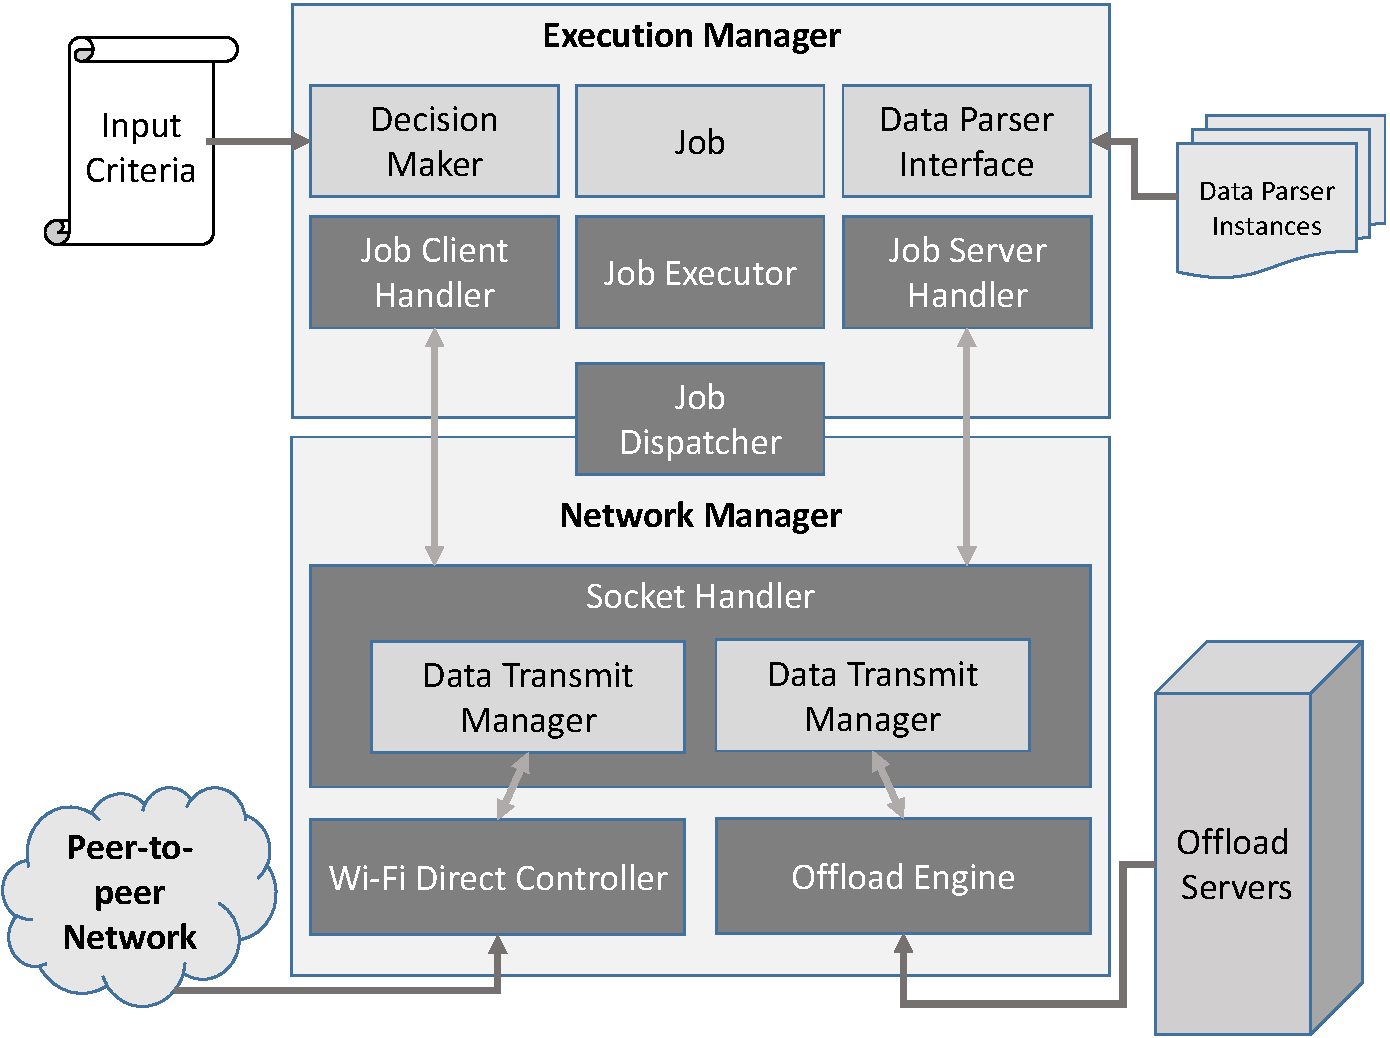
\includegraphics[width=0.39\textwidth, natwidth=643, natheight=559]{data/jobShareArch}
}
\end{figure}

\subsection{APIs for Peer-to-peer Network}
To easily establish connections between devices in the network, we utilized Wi-Fi Direct, the new feature available on Android 4.0 and later. \texttt{Wi-Fi Peer-to-peer Broadcaster} (WPB) module wraps up 

When the app starts up, WPB will call \texttt{discoverPeers()} to send a message to the other peers to let them know its availability. Once a peer receives such message, WPB will update the list of devices and reform the network


\begin{figure}[H]
\caption{Forming peer-to-peer network}
\centerline {
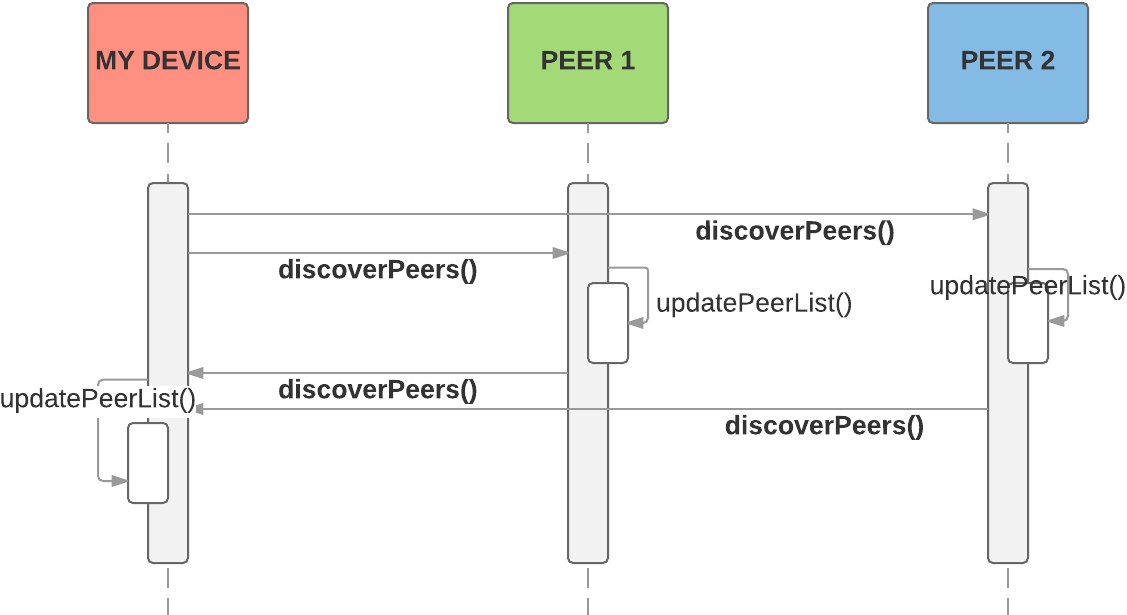
\includegraphics[width=0.5\textwidth, natwidth=1127, natheight=615]{data/discoverPeers}
}
\end{figure}

\subsection{Job definition}
The system should accept any kind of Job. To avoid any mistakes in remote execution, we provide an united Job interface

\begin{lstlisting}[caption=Job Definition]
public class Job {
	public Object exec(Object originalObject) {
		// job implementation
	}
}
\end{lstlisting}

Since Android SDK doesn't support call 


\section{Experiments}

\section{Conclusions}
The conclusion goes here.




% conference papers do not normally have an appendix


% use section* for acknowledgment
\section*{Acknowledgment}


The authors would like to thank...





% trigger a \newpage just before the given reference
% number - used to balance the columns on the last page
% adjust value as needed - may need to be readjusted if
% the document is modified later
%\IEEEtriggeratref{8}
% The "triggered" command can be changed if desired:
%\IEEEtriggercmd{\enlargethispage{-5in}}

% references section

% can use a bibliography generated by BibTeX as a .bbl file
% BibTeX documentation can be easily obtained at:
% http://mirror.ctan.org/biblio/bibtex/contrib/doc/
% The IEEEtran BibTeX style support page is at:
% http://www.michaelshell.org/tex/ieeetran/bibtex/
%\bibliographystyle{IEEEtran}
% argument is your BibTeX string definitions and bibliography database(s)
%\bibliography{IEEEabrv,../bib/paper}
%
% <OR> manually copy in the resultant .bbl file
% set second argument of \begin to the number of references
% (used to reserve space for the reference number labels box)
\begin{thebibliography}{100}

\bibitem{rbnb}
Sameer Tilak, Paul Hubbard, Matt Miller, and Tony Fountain, \emph{The Ring Buffer Network Bus (RBNB) DataTurbine Streaming Data Middleware for Environmental Observing Systems}, p125-133, e-Science and Grid Computing, Bangalore 2007.

\bibitem{rabbitmq}
Maciej Rostanski, Krzysztof Grochla, Aleksander Seman, \emph{Evaluation of highly available and fault-tolerant
middleware clustered architectures using RabbitMQ}, p879-884, FedCSIS 2014.

\bibitem{naradabrokering}
Gadgil, H.; Fox, G.; Pallickara, S.; Pierce, M. \emph{Managing grid messaging middleware}, Challenges of Large Applications in Distributed Environments, p83-91, 2006 IEEE

\end{thebibliography}



% that's all folks
\end{document}


